\chapter{前端项目}

\section{设计}
\subsection{项目相关知识点}
\subsubsection{屏幕视口}
移动端的屏幕尺寸非常多样,而不像~PC~端的屏幕那样一致。因此,在移动设备上显示网页时,由于尺寸的不同,可能会出现网页内容显示不全且需要横向滚动的情况,因此在本软件运用了屏幕视口(viewport)的功能。

屏幕视口可分为三种,分别为:
\begin{enumerate}
    \item{布局视口(layout viewport)}:网页的实际尺寸。
    \item {理想视口(ideal viewport)}:网页在屏幕上的实际尺寸,根据机型的不同,尺寸也不尽相同。
    \item {视觉视口(visual viewport)}:用户所能看到的视口范围。
\end{enumerate}

通过使用屏幕视口(viewport),可以有效解决上述的问题:将网页放置在布局视口(layout viewport)中,然后按比例缩小布局视口以适应理想视口(ideal viewport)。这样可以确保无论网页的内容如何,都能在移动设备的屏幕上完整显示,而且不会出现横向滚动条的情况。

在每次开发网页前,我们会在头部加上一段屏幕视口的代码,代码如下:
\begin{lstlisting}[basicstyle=\footnotesize]
<meta name="viewport" content="width=device-width, initial-scale=1">
\end{lstlisting}
其中,~width~是布局视口,而~device-width~理想尺寸。因此,~width=device-width~就是将布局视口按照理想视口的实际尺寸来显示。

\subsubsection{弹性布局}
在此项目中,我们会将某些元素(div)的~display~属性值设置为~flex~,那么这个元素就可以称为是一个弹性布局容器(弹性容器)。它的子元素将会按照弹性布局的规则来排列和对齐。
\begin{lstlisting}[basicstyle=\footnotesize]
display: flex
\end{lstlisting}

在弹性布局中,默认存在着两根轴,分别是水平方向的主轴和垂直方向的侧轴。如图~\ref{fig:axis}~所示。
\begin{figure}[htbp]
    \centering
    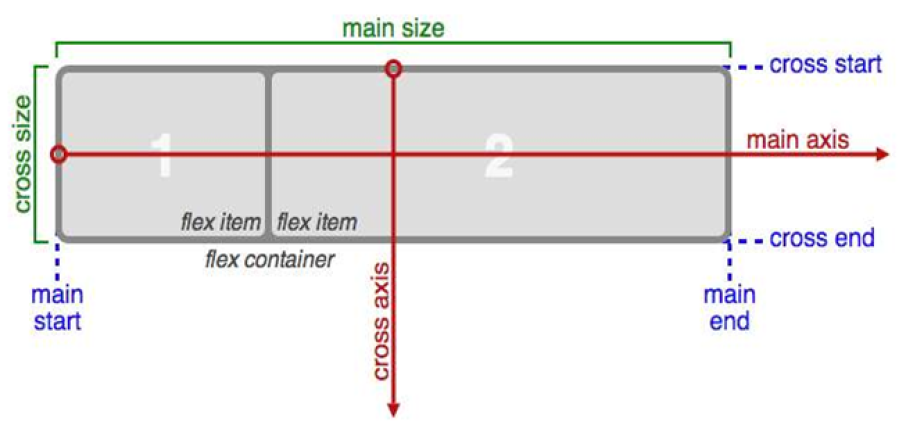
\includegraphics[width=0.8\textwidth]{axis}
    \caption{弹性布局的主轴与侧轴}\label{fig:axis}
    \vspace{\baselineskip}
\end{figure}

我们使用~flex-direction~属性来设置主轴的方向,row~为主轴方向且为默认值,而column~为侧轴方向。
\begin{lstlisting}[basicstyle=\footnotesize]
flex-direction: column
\end{lstlisting}

由于弹性布局中的子元素能自动伸缩,因此当父容器的尺寸小于子元素整体尺寸时,子元素会自动收缩,而不是自动换行。如果向让子元素自动换行,需要使用~flex-wrap: wrap。
\begin{lstlisting}[basicstyle=\footnotesize]
display: flex
flex-wrap: wrap
\end{lstlisting}

在此项目中,我们会设置 justify-content 样式,让子元素水平居中、居右等等。其中,justify-content 有五种值:
\begin{enumerate}
    \item{flex-start}:居左,为默认值。
    \item {flex-end}:居右。
    \item {center}:居中。
    \item {space-between}:两端对齐,每个子元素的间距相等。
    \item {space-around}:每个子元素两侧的间距相等。
\end{enumerate}
\begin{lstlisting}[basicstyle=\footnotesize]
display: flex
justify-content: space-between
\end{lstlisting}

除了让子元素水平居中、居右等,我们还使用了 align-items 样式,以让子元素垂直居中。
\begin{lstlisting}[basicstyle=\footnotesize]
display: flex
align-items: center
\end{lstlisting}

为了让每个子元素所占空间不一致,我们也使用 flex 样式给子元素按比例分配空间。如果设置了 flex,width 与 height 就会失效。
\begin{lstlisting}[basicstyle=\footnotesize]
<body>
    <div class="son" style="flex:1;">1</div>
    <div class="son" style="flex:1;">2</div>
    <div class="son" style="flex:2;">3</div>
</body>
\end{lstlisting}
在上面例子中,三个 div 的宽度分别是窗口宽度的 1/4、1/4 和 1/2。
\begin{lstlisting}[basicstyle=\footnotesize]
<body>
    <div class="son" style="flex:0 0 400px;">1</div>
    <div class="son" style="flex:1;">2</div>
    <div class="son" style="flex:2;">3</div>
</body>
\end{lstlisting}
在上面例子中,第一个 div 的宽度是 400px,是不变的。第二个和第三个 div 将剩下宽度按比例分配:1/3、2/3。

在移动端中,视口指的是屏幕视口中的布局视口。视口尺寸常用的有 vw 和 vh。1vw 等于视口宽度的1\%,而 1vh 等于视口高度的1\%。在此项目中,我们会多使用 vw,以实现元素宽度按移动端当前的宽度自动缩放。
\begin{lstlisting}[basicstyle=\footnotesize]
<style>
    div{
        width: 30vw;
        height: 20vw;
        background-color: blue;
        color: #fff;
        font-size: 5vw;
    }
</style>
\end{lstlisting}

CSS3 新增了 border-box 的盒子模型,即宽和高为边框。我们使用 box-sizing 的属性来设置盒子模型类型。使用了边框盒子后,就可以任意设置内边距、边框,不需要担心会改变盒子的总体尺寸。
\begin{lstlisting}[basicstyle=\footnotesize]
div{
    width: 200px;
    height: 200px;
    box-sizing: border-box; 
    padding: 30px;
    border: solid 30px blue;
    margin: 50px;
}
\end{lstlisting}
private Integer foodId;
private String foodName;
private String foodExplain;
private Double foodPrice;
private Integer businessId;private Integer foodId;
private String foodName;
private String foodExplain;
private Double foodPrice;
private Integer businessId;
\subsection{项目搭建}
本项目为前端静态页面项目,一共制作 15 个不同的页面,分别为:
\begin{enumerate}
    \item{首页}
    \item {商家列表页面}
    \item {商家信息页面}
    \item {确认订单页面}
    \item {在线支付页面}
    \item {支付成功页面}
    \item {历史订单页面}
    \item {地址管理页面}
    \item {新增地址页面}
    \item {编辑地址页面}
    \item {用户登录页面}
    \item {用户注册页面}
    \item {个人信息页面}
    \item {更新用户名页面}
    \item {更新密码页面}
\end{enumerate}

本项目可分为三个部分,分别为相应页面的 HTML 部分、CSS 部分和 JavaScript 三个部分。在项目文件中,也存放了 framework 文件和 img 文件,前者为存放第三方库字体图标库以及 CSS 重置文件;后者则为存放网页所需要插入的一些图片。本项目的文件如图~\ref{fig:part2folder}~所示。

我们使用了 font-awesome 作为本软件的第三方字体图标库,让我们可以插入各种不同的图标,以增加用户对于本软件的视觉效果。Font-awesome 第三方字体图标库网页如图~\ref{fig:fontawesomeweb}~所示。

创建 CSS 重置文件主要是为了去除 CSS 默认的边角、列表样式以及超链接下划线,代码如下:
\begin{lstlisting}[basicstyle=\footnotesize]
/* ----------------CSS 重置-------------- */
html, body, div, span, h1, h2, h3, h4, h5, h6, ul, ol, li, p{
    margin: 0;
    padding: 0;
}
/* 将边角去掉 */
html, body{
    height: 100%;
    weight: 100%;
    font-family: "微软雅黑";
}
/* 去掉列表样式 */
ul,ol{
    list-style: none;
}
/* 去掉超链接下划线 */
a{
     text-decoration: none;
}
\end{lstlisting}
\begin{figure}[htbp]
    \centering
    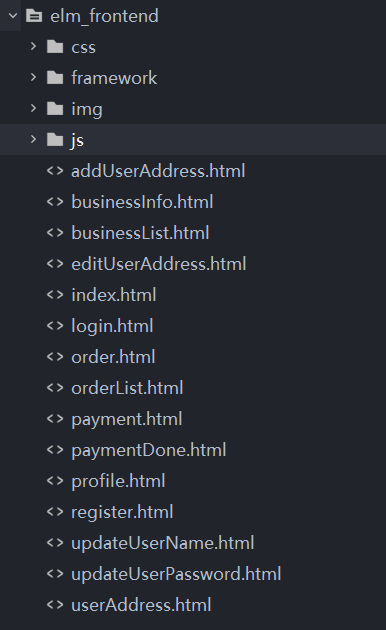
\includegraphics[width=0.4\textwidth]{part2folder}
    \caption{项目结构}\label{fig:part2folder}
    \vspace{\baselineskip}
\end{figure}
\begin{figure}[htbp]
    \centering
    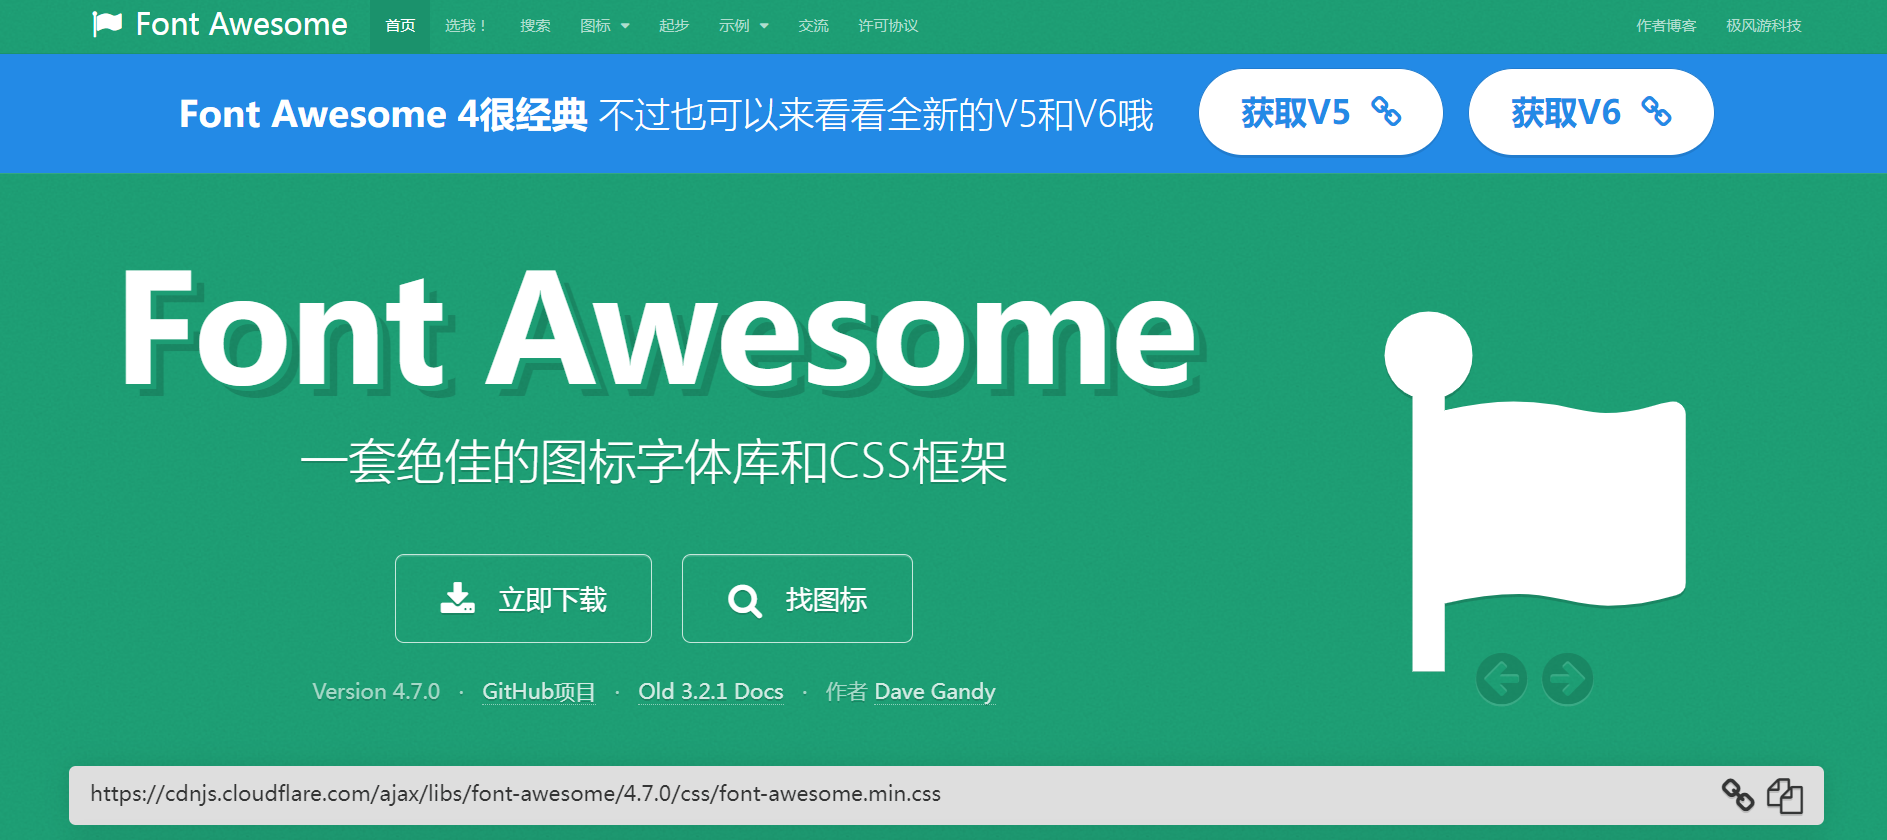
\includegraphics[width=0.8\textwidth]{fontawesomeweb}
    \caption{Font-awesome 网页}\label{fig:fontawesomeweb}
    \vspace{\baselineskip}
\end{figure}

\subsection{共通部分}
本软件的页面采用了共通的头部设计,因此在每个页面的 HTML 和 CSS 文件中都会包含这些共通部分的代码。
\subsubsection{页面头部}
对于每个页面,都采用了相同的页面头部,其中头部尺寸、背景色以及字体都是相同的。因此,在每个页面的 HTML 文件和 CSS 文件都会包含以下代码:
\begin{lstlisting}[basicstyle=\footnotesize]
/***** HTML 部分 *****/
<header><p>商家列表</p></header>

/***** CSS 部分 *****/
.wrapper header{
	width: 100%;
	height: 12vw;
	background-color: deepskyblue;
	position: fixed;
	top: 0;
	left: 0;
	display: flex;
	justify-content: center;
	align-items: center;
	color: white;
	font-size: 5vw;
	font-weight: 700;
}
\end{lstlisting}    
以上代码的生成结果如图~\ref{fig:headerfix}~所示。
\begin{figure}[htbp]
    \centering
    
\includegraphics[width=0.8\textwidth]{headerfix}
    \caption{页面头部界面设计}\label{fig:headerfix}
    \vspace{\baselineskip}
\end{figure}

\subsubsection{底部菜单}
除了商家列表页面、商家信息页面以及支付成功页面,对于每个页面也采用了相同的底部菜单设计。该底部菜单固定在屏幕的底部,但不会独占整个底部,而是稍微向上腾出一点空间,给予底部菜单一种悬浮的视觉效果。

因此,在这些页面的 HTML 和 CSS 文件中都会包含以下代码:
\begin{lstlisting}[basicstyle=\footnotesize]
/***** HTML 部分 *****/
<ul class="footer">
    <li onclick="location.href = 'index.html'">
        <i class="fa fa-home"></i>
        <p>首页</p>
    </li>
    <li>
        <i class="fa fa-compass"></i>
        <p>发现</p>
    </li>
    <li onclick="location.href = 'orderList.html'">
        <i class="fa fa-file-text"></i>
        <p>订单</p>
    </li>
    <li onclick="location.href = 'profile.html'">
        <i class="fa fa-user"></i>
        <p>我的</p>
    </li>
</ul>

/***** CSS 部分 *****/
.wrapper .footer{
	width: 95%;
	height: 14vw;
	border: solid 1.5px darkgray;
	background-color: white;
	border-radius: 5vw;
	position: fixed;
	bottom: 3vw;
	left: 2.5%;
	display:flex;
	justify-content: space-around;
	align-items: center;
}
.wrapper .footer li{
	display:flex;
	flex-direction: column;
	align-items: center;
	justify-content: center;
	font-size:5vw;
	color: gray;
	user-select: none;
	cursor: pointer;
}
.wrapper .footer li p{
	font-size:2.8vw;
}
\end{lstlisting}
以上代码的生成结果如图~\ref{fig:footerfix}~所示。  
\begin{figure}[htbp]
    \centering
    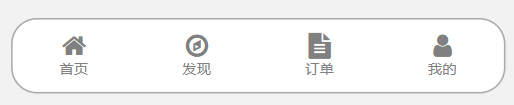
\includegraphics[width=0.8\textwidth]{footerfix}
    \caption{页面底部菜单界面设计}\label{fig:footerfix}
    \vspace{\baselineskip}
\end{figure}

\subsection{固定块}
本软件的页面主要有两个部分为固定块,分别为页面的底部菜单和首页中的搜索框部分。

\subsubsection{底部菜单}
对于页面的底部菜单,我们在相应页面的 CSS 文件中的底部菜单部分添加了 position: fixed 来达到固定屏幕上的效果。此外,为了呈现居中以及悬浮的效果,也增加了一段 left: 2.5\% 和 bottom: 3vw,其作用是为了让底部菜单向左保持 2.5\% 的间距以及向上移动 3vw。代码如下:
\begin{lstlisting}[basicstyle=\footnotesize]
position: fixed;
bottom: 3vw;
left: 2.5%;
\end{lstlisting}

\subsubsection{首页搜索框}
对于首页的搜索框部分,如果页面向下滑动,需要呈现出搜索框始终固定在头部的效果。这需要使用到 JavaScript 为搜索框写出一段逻辑代码。

我们使用了 onscroll 事件为固定搜索框创建一个函数。首先,我们获取滚动条的位置,获取PC端滚动条位置为 document.documentElement.scrollTop,而获取移动端滚动条位置为 document.body.scrollTop。由于 PC 端和移动端的获取方法有所不同,因此我们对它们做出了一个判断,如果从 PC 端获取的返回结果不为 0 则使用 PC 端的滚动条位置,否则使用移动端的滚动条位置。

接着,使用 document.documentElement.clientWidth 来获取视口的宽度,这对 PC 端和移动端都有效,然后使用 document.getElementById('fixedBox') 获取搜索框块。最后,写出一个判断:如果滚动条的位置大于首页头部的高度(12 vw),则将搜索框转换成固定,即写为 position: fixed;否则搜索框保持不变。代码如下:
\begin{lstlisting}[basicstyle=\footnotesize]
document.onscroll = function(){
    //获取滚动条位置
    let s1 = document.documentElement.scrollTop;
    let s2 = document.body.scrollTop;
    let scroll = s1==0?s2:s1; //判断是否是移动端或PC端
    //获取视口宽度
    let width = document.documentElement.clientWidth;
    //获取固定块
    let search = document.getElementById('fixedBox');
    if(scroll > width * 0.12){ //因为header的高度是 12vw
        search.style.position = 'fixed';
        search.style.left = '0';
        search.style.top = '0';
    }
    else{
        search.style.position = 'static';
    }
}
\end{lstlisting}
以上代码的执行效果如图~\ref{fig:searchnonfix}~和图~\ref{fig:searchfix}~所示。
\begin{figure}[htbp]
    \centering
    \begin{minipage}{0.4\textwidth}
    \centering
    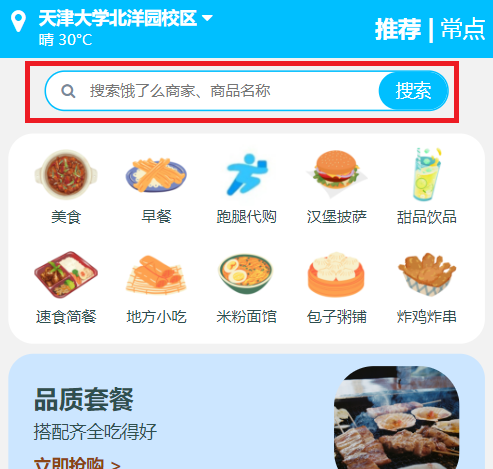
\includegraphics[width=\textwidth]{searchnonfix}
    \caption{首页无滚动时的搜索框}\label{fig:searchnonfix}
    \end{minipage}
    \begin{minipage}{0.4\textwidth}
    \centering
    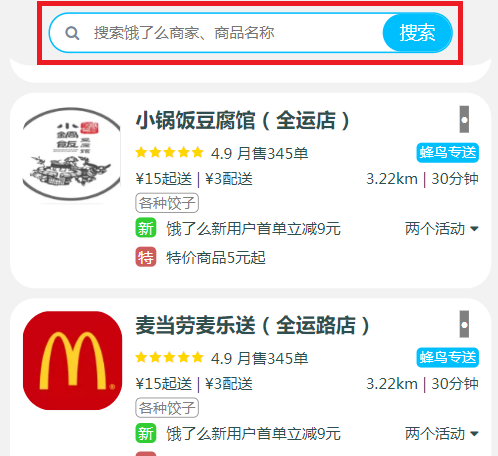
\includegraphics[width=\textwidth]{searchfix}
    \caption{首页滚动后的搜索框}\label{fig:searchfix}
    \end{minipage}
    \vspace{\baselineskip}
\end{figure}

\subsection{订单明细的显示与隐藏}
本软件有两个页面需要显示和隐藏外卖订单的明细,分别为确认订单页面以及历史订单页面。

首先,使用 document.getElementsByClassName('fa-caret-down') 和 document.getElementsByClassName('order-detail') 获取按钮和订单明细的对象。接着,使用 detailBox.style.display='none' 来初始化订单明细为隐藏状态。

最后,使用 onclick 事件为显示和隐藏订单明细的按钮创建一个函数。在函数里写出一个判断:如果当前订单明细为隐藏状态,则当点击按钮时会显示订单明细;否则点击按钮时会隐藏订单明细。代码如下:
\begin{lstlisting}[basicstyle=\footnotesize]
//获取显示隐藏按钮对象
let downBtn  = document.getElementsByClassName('fa-caret-down');
//获取隐藏订单明细对象
let detailBox = document.getElementsByClassName('order-detail');
//所有订单明细初始为隐藏状态
for(let i = 0; i < downBtn.length; i++){
    detailBox[i].style.display='none';
}
for(let i = 0; i < downBtn.length; i++){
    downBtn[i].onclick = function(){
        //判断隐藏订单明细是否隐藏
        if(detailBox[i].style.display=='none'){
            detailBox[i].style.display='block';
        }
        else{
            detailBox[i].style.display='none';
        }
    }
}
\end{lstlisting}
以上代码的执行效果如图~\ref{fig:orderhidden}~和图~\ref{fig:ordershown}~所示。
\begin{figure}[htbp]
    \centering
    \begin{minipage}{0.4\textwidth}
    \centering
    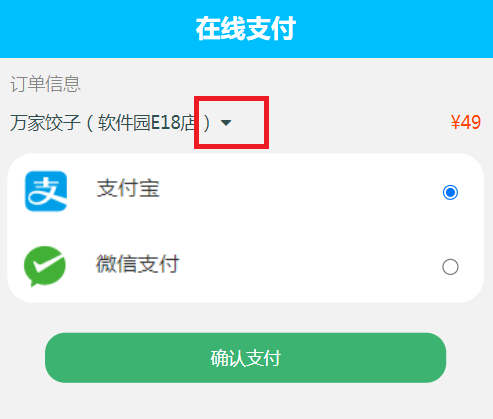
\includegraphics[width=\textwidth]{orderhidden}
    \caption{订单明细隐藏状态}\label{fig:orderhidden}
    \end{minipage}
    \begin{minipage}{0.4\textwidth}
    \centering
    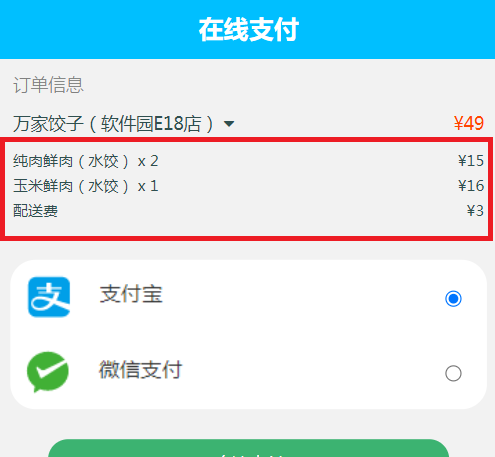
\includegraphics[width=\textwidth]{ordershown}
    \caption{订单明细显示状态}\label{fig:ordershown}
    \end{minipage}
    \vspace{\baselineskip}
\end{figure}

\section{测试}
对于本项目的测试,主要着重于每个页面的按钮是否能跳转至正确的页面,以及对于某些页面的逻辑操作是否正确。

\subsection{页面按钮测试}
对于页面按钮的测试,首先测试每个页面的底部菜单按钮是否都可以跳转至相应的页面。如果点击 “首页” 则必须跳转至首页;点击 “发现” 则没有任何效果;点击 “订单” 则必须跳转至历史订单页面;点击 “我的” 则必须跳转至个人信息页面。

经过测试,每个设计底部菜单的页面都可以正常跳转至指定的页面,如图~\ref{fig:part2test}~所示。
\begin{figure}[htbp]
    \centering
    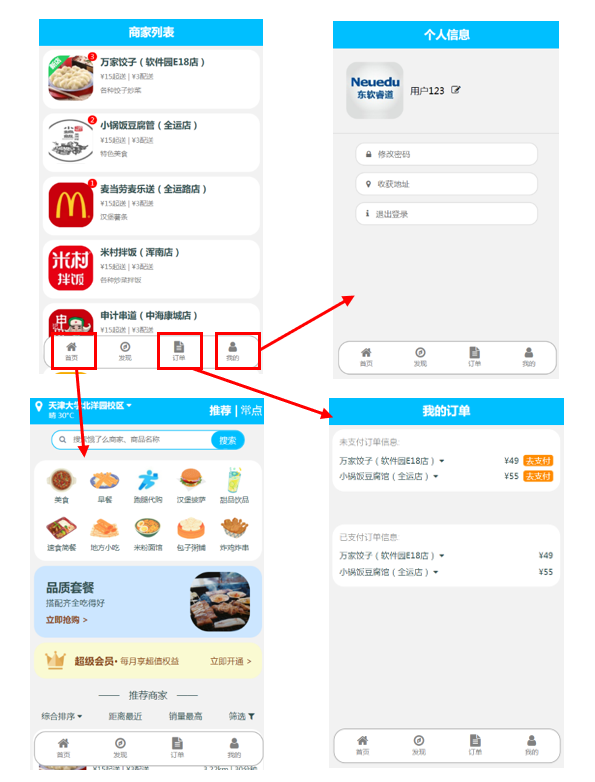
\includegraphics[width=0.5\textwidth]{part2test}
    \caption{页面底部菜单按钮测试}\label{fig:part2test}
    \vspace{\baselineskip}
\end{figure}

接着我们测试了其余页面的其他按钮是否可以正确跳转至相应的页面。由于本软件的按钮过多,因此在本项目的测试部分只显示首页、地址管理页面和个人信息页面的按钮测试结果,如图~\ref{fig:part2test1}~和图~\ref{fig:part2test2}~所示。
\begin{figure}[htbp]
    \begin{minipage}{0.6\textwidth}
    \centering
    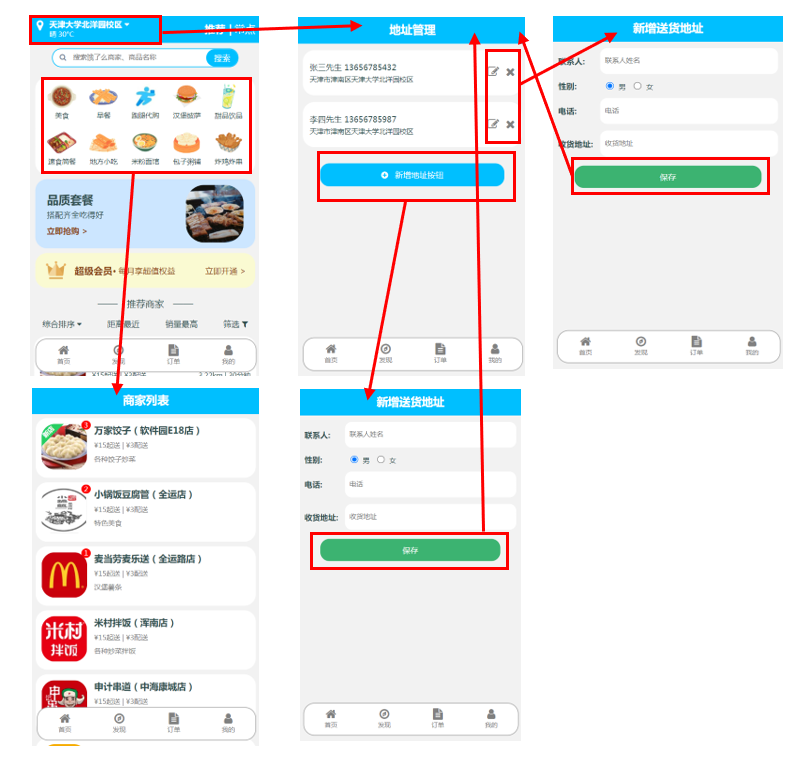
\includegraphics[width=\textwidth]{part2test1}
    \caption{首页和地址管理页面按钮测试}\label{fig:part2test1}
    \end{minipage}
    \begin{minipage}{0.5\textwidth}
    \centering
    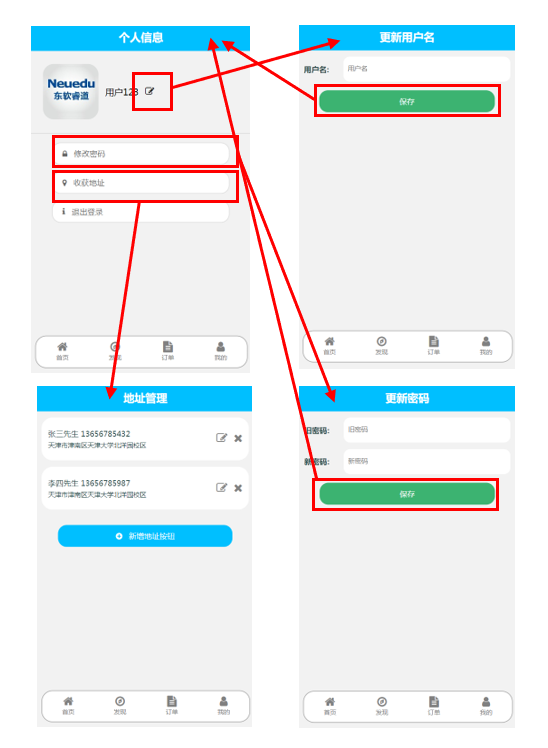
\includegraphics[width=\textwidth]{part2test2}
    \caption{个人信息页面按钮测试}\label{fig:part2test2}
    \end{minipage}
    \vspace{\baselineskip}
\end{figure}

\subsection{页面逻辑操作}
在本项目中需要对逻辑操作进行测试的页面有首页、确认订单页面与历史订单页面。对于首页,我们所需要测试的是搜索框在页面向下滑动时是否会固定在页面头部,测试结果如图~\ref{fig:part2test3}~和图~\ref{fig:part2test4}~所示。
\begin{figure}[htbp]
    \centering
    \begin{minipage}{0.4\textwidth}
    \centering
    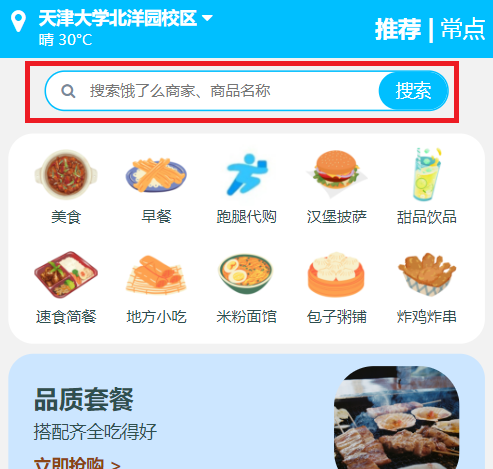
\includegraphics[width=\textwidth]{searchnonfix}
    \caption{首页无滚动时的搜索框}\label{fig:part2test3}
    \end{minipage}
    \begin{minipage}{0.4\textwidth}
    \centering
    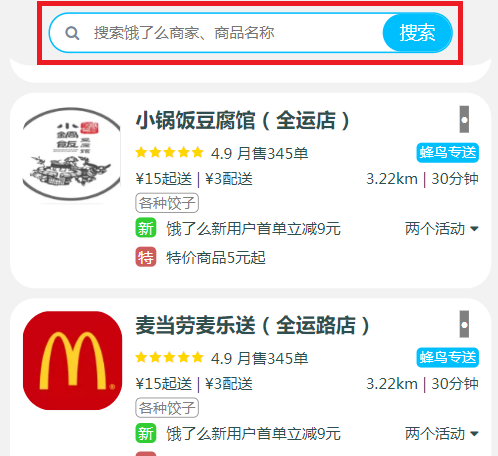
\includegraphics[width=\textwidth]{searchfix}
    \caption{首页滚动后的搜索框}\label{fig:part2test4}
    \end{minipage}
    \vspace{\baselineskip}
\end{figure}

接着,对于确认订单页面和历史订单页面,我们测试了这两个页面是否可以正确显示和隐藏订单,且在初始状态时为隐藏状态。测试结果如图~\ref{fig:part2test5}~至~\ref{fig:part2test8}~所示。
\begin{figure}[htbp]
    \centering
    \begin{minipage}{0.4\textwidth}
    \centering
    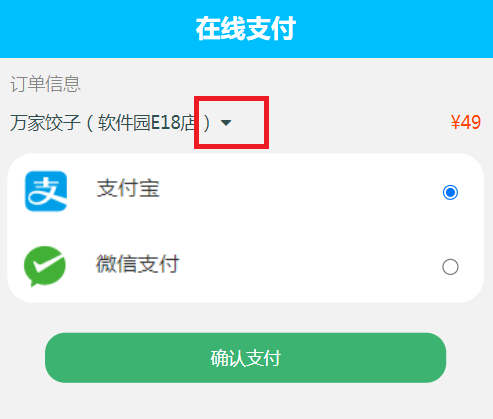
\includegraphics[width=\textwidth]{orderhidden}
    \caption{确认订单页面订单明细隐藏状态}\label{fig:part2test5}
    \end{minipage}
    \begin{minipage}{0.4\textwidth}
    \centering
    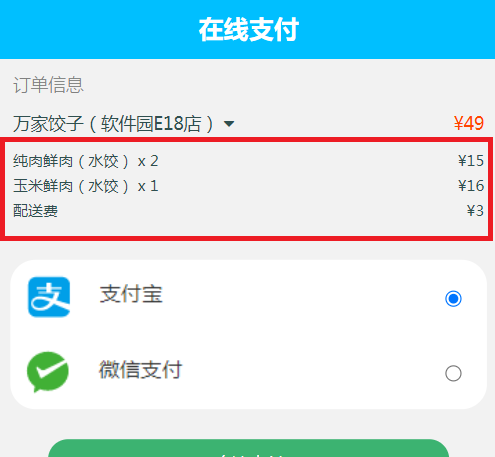
\includegraphics[width=\textwidth]{ordershown}
    \caption{确认订单页面订单明细显示状态}\label{fig:part2test6}
    \end{minipage}
    \vspace{\baselineskip}
\end{figure}
\begin{figure}[htbp]
    \centering
    \begin{minipage}{0.4\textwidth}
    \centering
    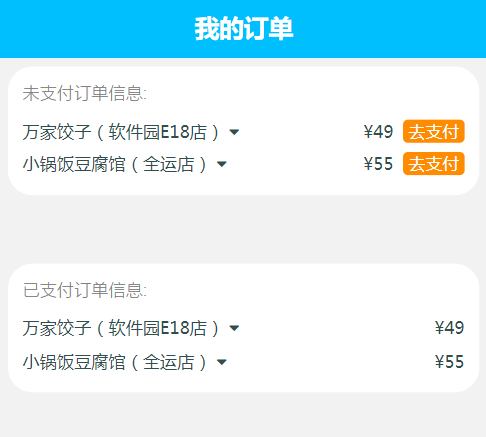
\includegraphics[width=\textwidth]{part2test7}
    \caption{历史订单页面订单明细隐藏状态}\label{fig:part2test7}
    \end{minipage}
    \begin{minipage}{0.4\textwidth}
    \centering
    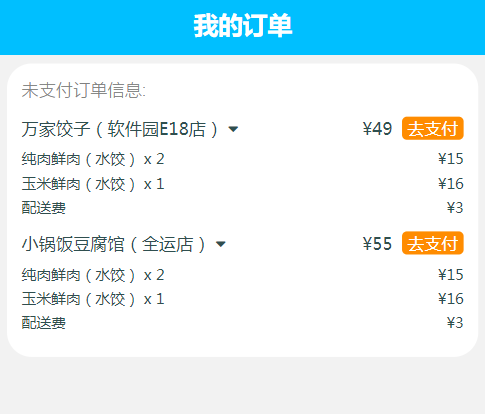
\includegraphics[width=\textwidth]{part2test8}
    \caption{历史订单页面订单明细显示状态}\label{fig:part2test8}
    \end{minipage}
    \vspace{\baselineskip}
\end{figure}